\documentclass[11pt, oneside]{article}   	% use "amsart" instead of "article" for AMSLaTeX format
\usepackage{geometry}                		% See geometry.pdf to learn the layout options. There are lots.
\geometry{letterpaper}                   		% ... or a4paper or a5paper or ... 
%\geometry{landscape}                		% Activate for rotated page geometry
%\usepackage[parfill]{parskip}    		% Activate to begin paragraphs with an empty line rather than an indent
\usepackage{graphicx}				% Use pdf, png, jpg, or eps§ with pdflatex; use eps in DVI mode							% TeX will automatically convert eps --> pdf in pdflatex		
\usepackage{amssymb}
\usepackage{amsmath}
\usepackage{pythonhighlight}
\usepackage[colorlinks = true,
            linkcolor = blue,
            urlcolor  = blue,
            citecolor = blue,
            anchorcolor = blue]{hyperref}

\newcommand{\changeurlcolor}[1]{\hypersetup{urlcolor=#1}}       
\graphicspath{ {./images/} }
\usepackage{chngcntr}
\usepackage{float}
\let\oldsubsection\subsection
\renewcommand{\subsection}{%
    \setcounter{equation}{0}%
    \oldsubsection%
}


%SetFonts


\title{Assignment 3}
\author{Nicholas Pysklywec}
%\date{}							% Activate to display a given date or no date

\begin{document}
\maketitle

\section{Edge Detection}

To make a gaussian filter,  a function was created that takes in filter size, and sigma, and outputs the gaussian kernel. We use this in each of the questions where we require a gaussian filter of a given length. To perform the convolution process, a function was created to perform convolution that takes two arguments, one is the filter array, the other the image. 

\subsection*{Part A} 

The gaussian filter function constructed was used to develop two 5X5 gaussian filters, one for $\sigma = 1,$ and $\sigma = 2$. The image provided is convolved with each filter respectively, and we end up with the following two images from this:

\begin{figure}[H]
  \noindent\makebox[\textwidth]{%
  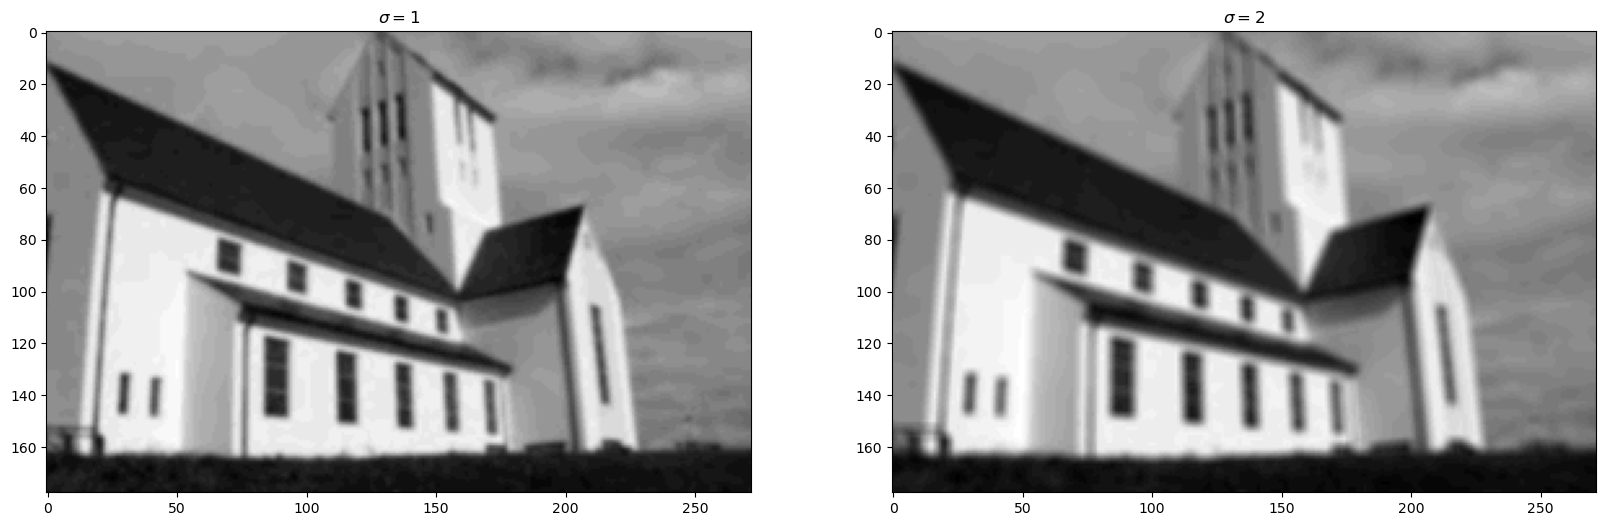
\includegraphics[width=1.2\textwidth]{1a}}
\end{figure}

\subsection*{Part B} 

We first construct 3x3 Sobel filters $S_x, S_y$, which look as follows:

\begin{equation*}
S_x = \begin{bmatrix}
   -1 &0 &1 \\
   -2 &0 &2 \\
   -1 &0 &1 \\
\end{bmatrix} \\
S_y = \begin{bmatrix}
   1 &2 &1 \\
   0 &0 &0 \\
   -1 &-2 &-1 \\
\end{bmatrix}
\end{equation*}

We convolve each of these filters to each of the images received in Part A. So first we perform this on the Gaussian $\sigma=1$ output:

\begin{figure}[H]
  \noindent\makebox[\textwidth]{%
  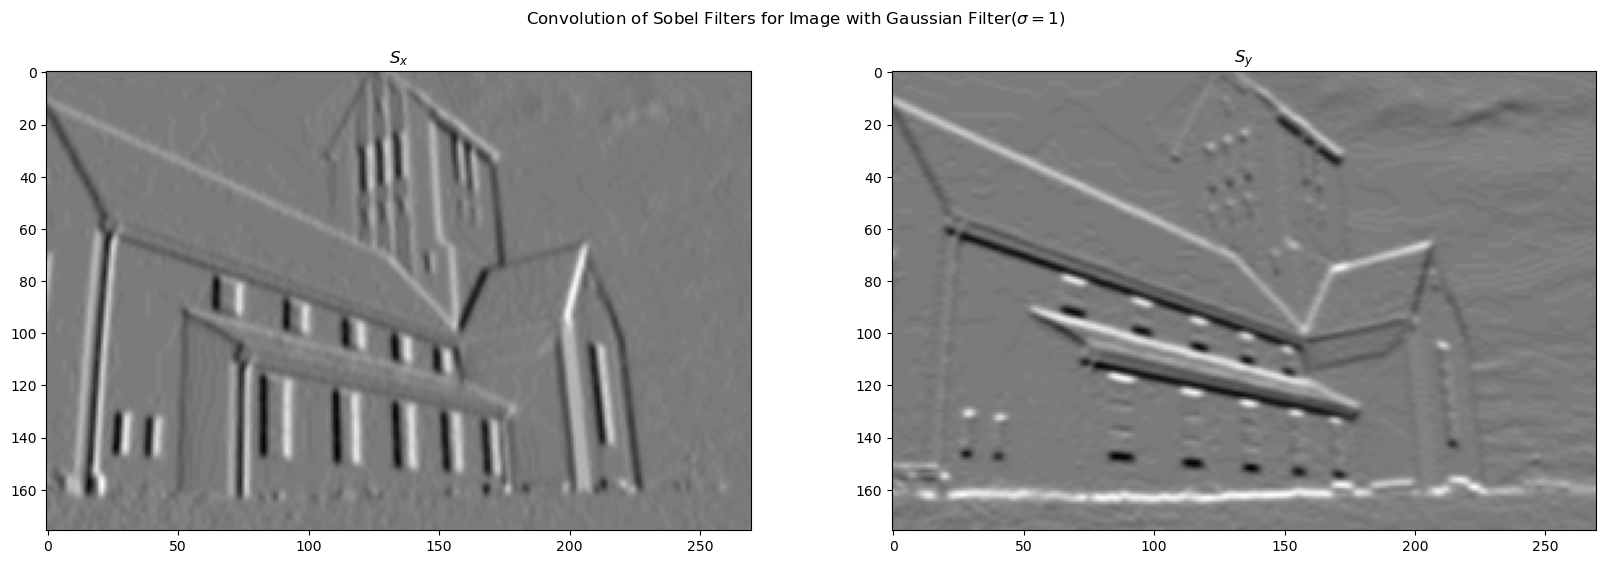
\includegraphics[width=1.2\textwidth]{1b1}}
\end{figure}
Then we convolve the Gaussian $\sigma=2$ with each Sobel filter:

\begin{figure}[H]
  \noindent\makebox[\textwidth]{%
  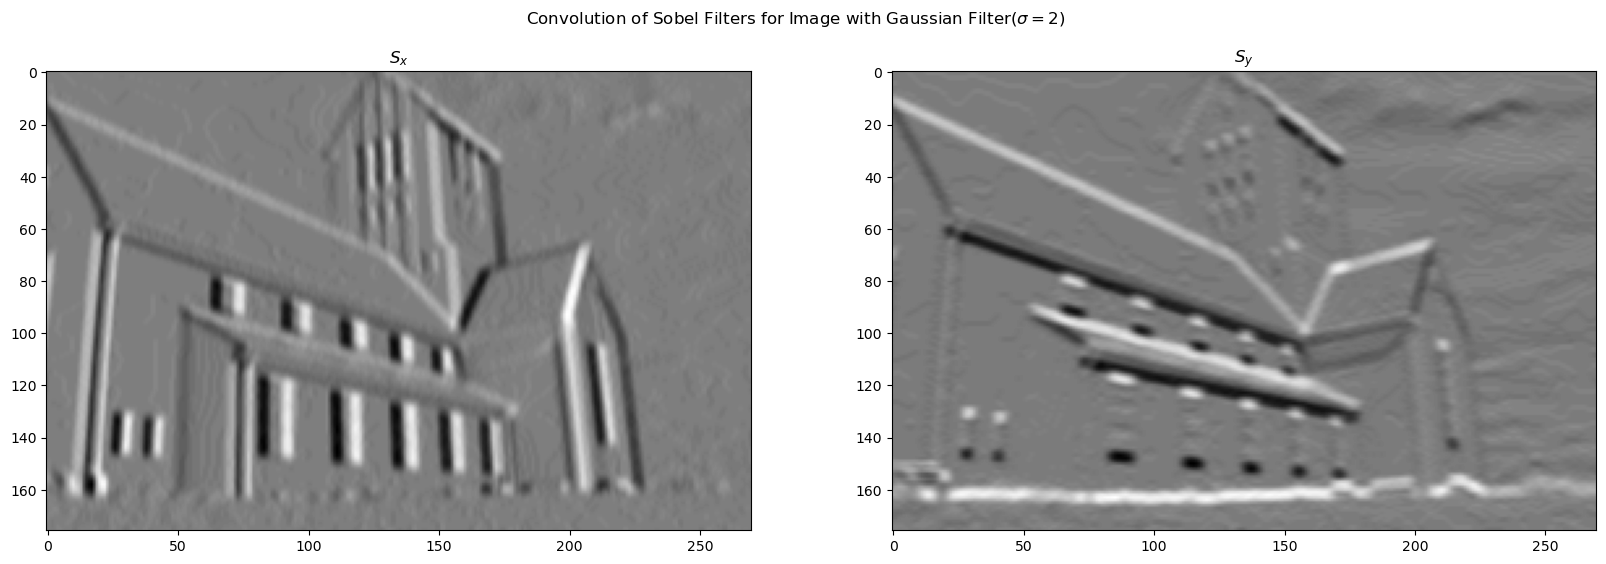
\includegraphics[width=1.2\textwidth]{1b2}}
\end{figure}

\subsection*{Part C}

We go back to the original image now, and make use of the $\frac{\delta G}{\delta x}, \frac{\delta G}{\delta y}$ filters. To obtain these filters, the Gaussian kernel function we defined earlier was remade to accompany the formula from the lectures.

We now convolve  $\frac{\delta G}{\delta x}$ and $\frac{\delta G}{\delta y}$ for value $\sigma = 1,$ and $2$:

\begin{figure}[H]
  \noindent\makebox[\textwidth]{%
  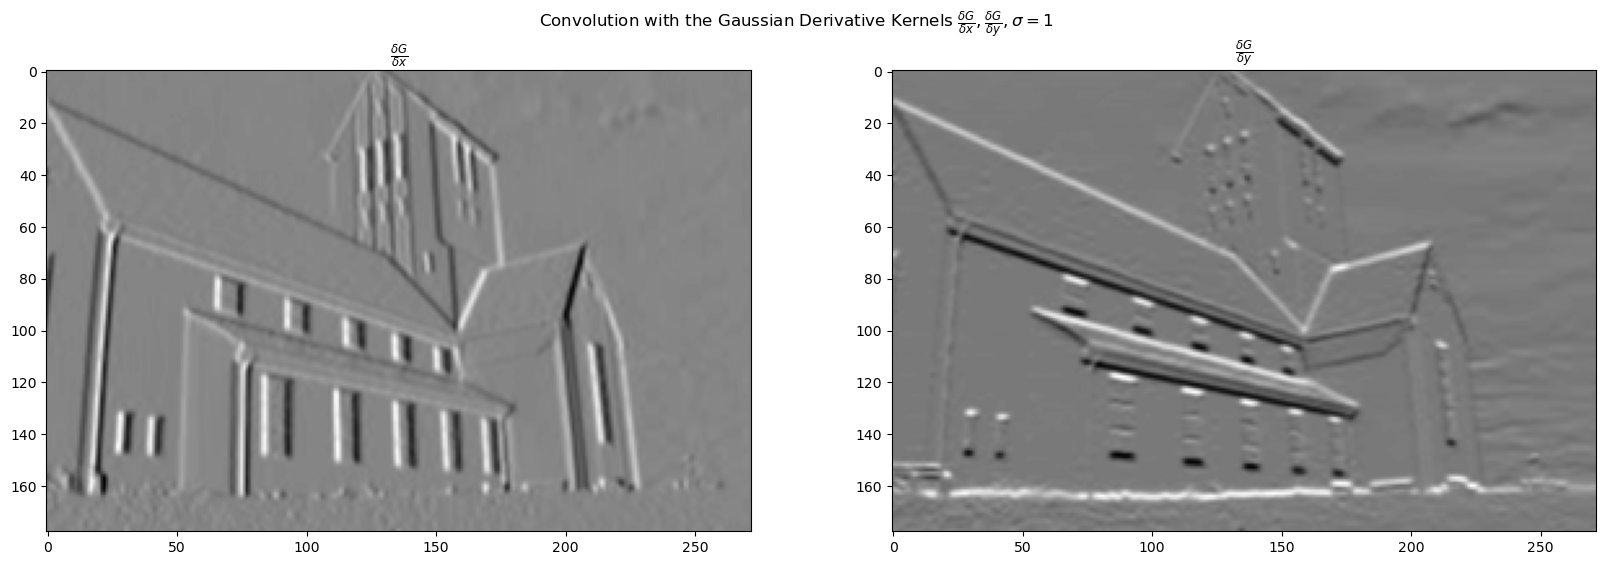
\includegraphics[width=1.2\textwidth]{1c1}}
  \end{figure}
\begin{figure}[H]
  \noindent\makebox[\textwidth]{%
  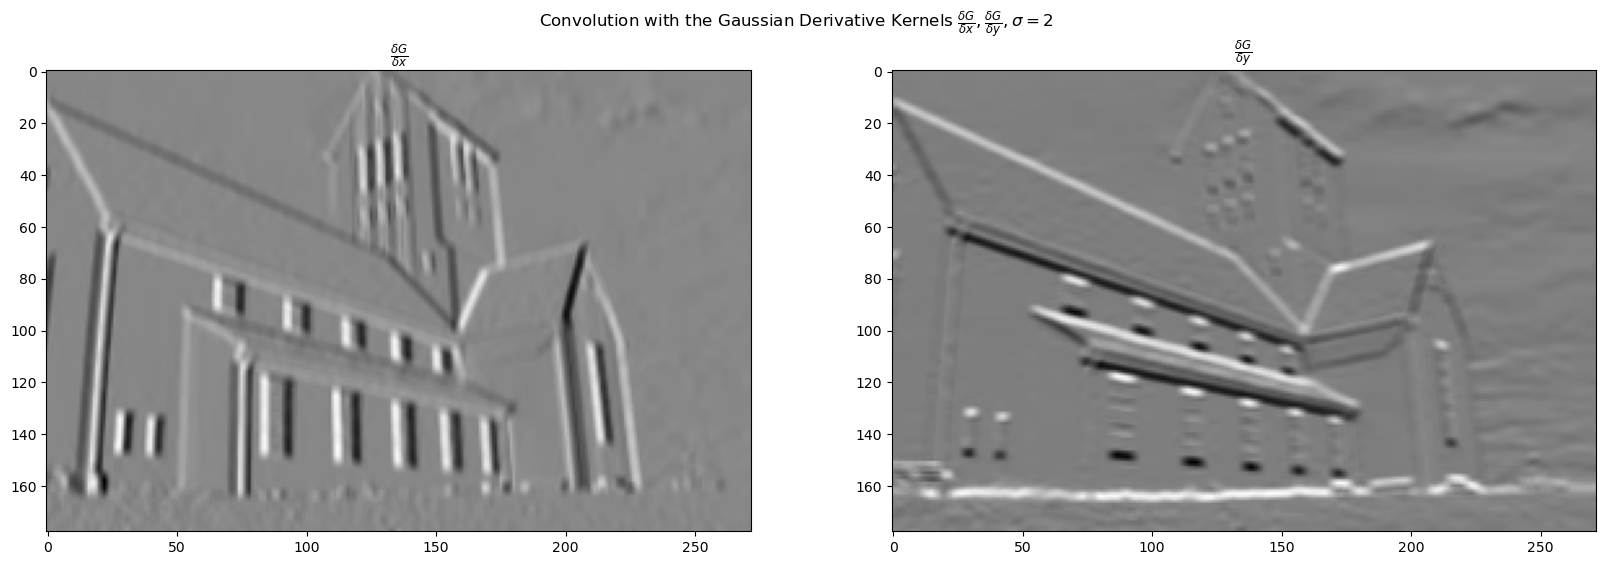
\includegraphics[width=1.2\textwidth]{1c2}}
\end{figure}

\subsection*{Explanation of B and C}
The images we received in Parts B and C are quite similar, however have a few differences still. Part B is Sobel operators with Gaussian filters, and these seem to really bring out the edges of the given direction(x for horizontal, y for vertical). As we increase $\sigma$ from 1 to 2, we only see the edge highlights become more pronounced. Now the Gaussian Derivatives used in Part C yield much more different results. Edges are highlighted, but not near the level the Sobel operators highlight edges. Instead what we see as we increae $\sigma$, the image becomes much more smooth. We can see that the Gaussian Derivative filters are likely best used for image smoothing cases. Sobel operators, alongside Gaussian filters can be used to highlight the edges in the images. Each pair of filters have their specific use case and specialty, that we can see in the above.


\section{Harris Corner Detection Implementation}

The Harris Corner Detection algorithm was implemented as presented in class. The original image was loaded in at grayscale. The spatial derivatives were calculated with use of the Sobel filters constructed in question 1b. The M tensor was then constructed. The window function $w$ used was a 3x3 gaussian filter.

\begin{equation*}
M(x,y) = \sum_{x,y} \in w\begin{bmatrix}
   I^2_x &I_xI_y \\
   I_xI_y & I^2_y\\
\end{bmatrix} 
\end{equation*}

These values were calculated. Finally the values of $M$ were used to determine the $R$ value. We used the following equation from class to do this, where $k = 0.04$:

\begin{equation*}
R = det(M) - k(traceM)^2
\end{equation*}

This provided the Harris Response values per pixel, which could be used with thresholding to determine corners, of images. We can map the Harris Corner response below:

\begin{figure}[H]
  \noindent\makebox[\textwidth]{%
  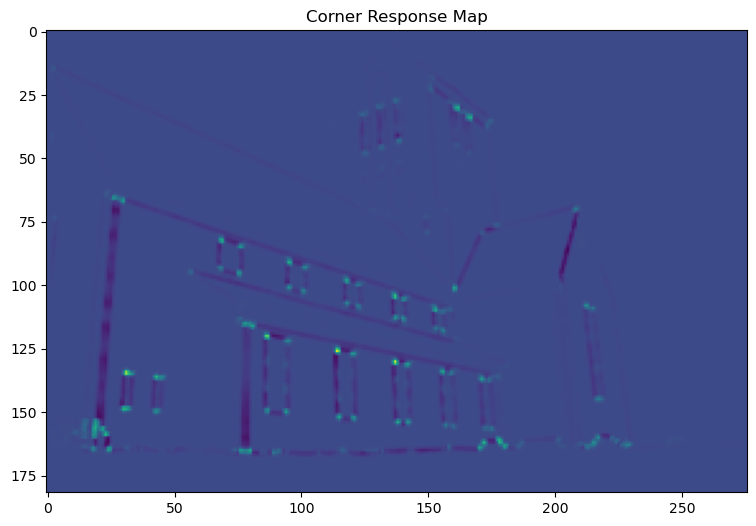
\includegraphics[width=1.2\textwidth]{32}}
\end{figure}

The map above demonstrates the utility of the Harris Response. We can see the general structure of the image, with corners being specifically singled out which is what is desired here.

The threshold used was dependent on the image, here we did:

\begin{equation*}
threshold = max(\text{Harris Response Values}) * 0.1
\end{equation*}

If we get the initial image, and draw dots on positions that have Harris Response above the threshold, we can end up with:

\begin{figure}[H]
  \noindent\makebox[\textwidth]{%
  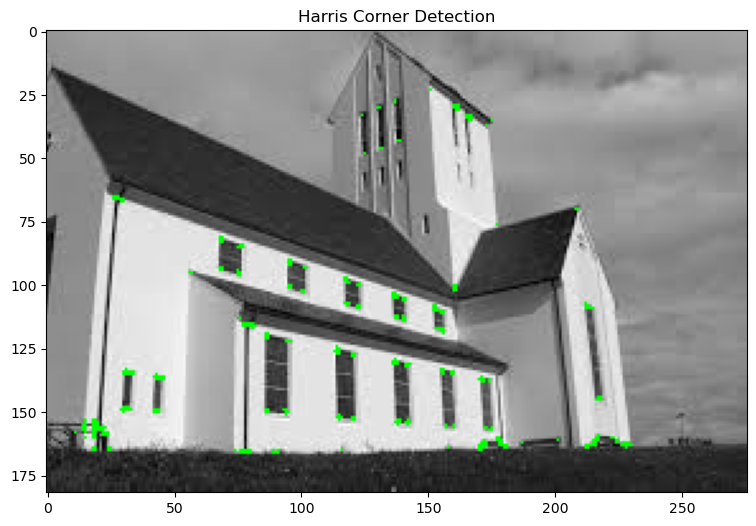
\includegraphics[width=1.2\textwidth]{31}}
\end{figure}

\end{document}  